\section{Q4} 

\subsection{Introduction} \label{sec:Introduction}

Freight elevators are essential systems in industrial and commercial environments, providing reliable 
vertical transportation of materials between different levels of a facility. In this laboratory exercise, 
the goal is to design and implement an electromagnetic control system to automate the operation of a freight 
elevator, using a three-phase motor managed by contactors and safety devices.

The proposed system must fulfill a specific set of operational requirements, including conditional 
upward and downward movement, timed delays, and immediate interruption in case of an emergency stop. 
Additionally, the system incorporates status indicators, such as lamps and sirens, to enhance operational 
safety and monitoring.

This report details the development of the control strategy through a Grafcet diagram, capturing the 
sequence of states and transitions governing the elevator’s operation. From this, the assembly diagram 
is created, illustrating the interconnections between all components and their terminal numbering. The 
electrical power and command circuits are subsequently derived and implemented in Fluidsim 3.6, enabling 
simulation and validation of the system’s compliance with the defined specifications.

The exercise reinforces critical concepts in industrial control, including the integration of safety 
mechanisms, timed operations, and the coordination of electrical and pneumatic components within an 
automated process.

\subsection{Grafcet Representation} \label{sec:Grafcet_Representation}

A structured graphical representation of the automation sequence is developed using the 
Grafcet method. This step-by-step graphical model illustrates the transitions between 
different states of the system, ensuring a clear understanding of the control logic.

\begin{figure}[H]
    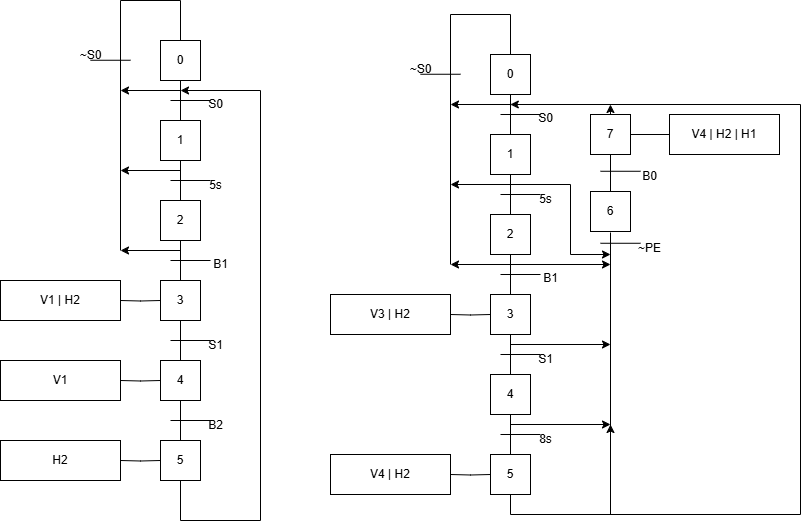
\includegraphics[width=16cm]{Images/Q4/graftset.png}
    \centering
    \caption{Grafset for the freight elevator}
    \label{fig:grafset}
\end{figure}

The Grafcet diagram presents a structured graphical representation of the automation sequence. It clearly defines 
the different states and transitions of the system, offering an intuitive 
understanding of how the automation logic operates based on the control loop described in Section \ref{sec:Control_Loop_Architecture}.

\subsection{Simulation and Validation} \label{sec:Simulation_and_Validation}

The final stage involves simulating the closed-loop control system in Fluidism 3.6 software. 
The simulation tests the interaction between the automation process, sensors, and actuators, 
validating whether the system meets the defined specifications. Any deviations are analyzed, 
and necessary modifications are proposed to optimize system performance.

\begin{figure}[H]
    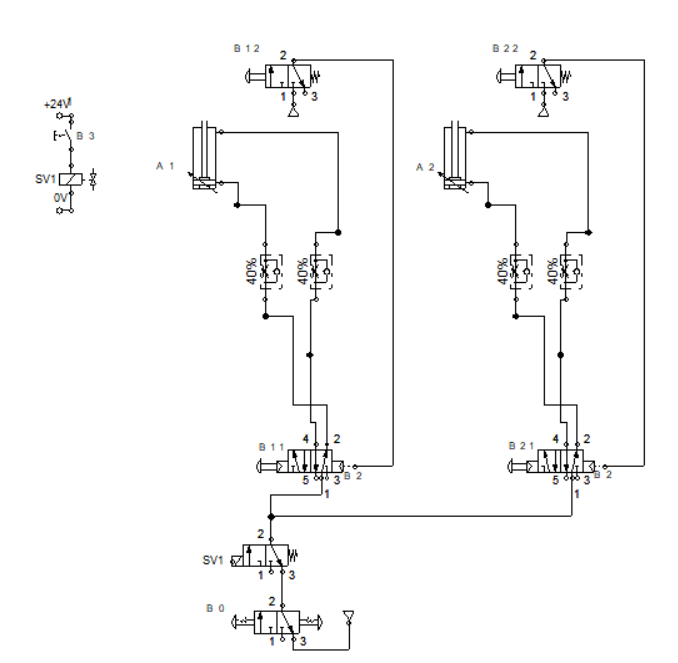
\includegraphics[width=16cm]{Images/Q4/fluidsim.png}
    \centering
    \caption{Fluidsim for the cargo elevator}
    \label{fig:fluidsim}
\end{figure}

The complete implementation of the control system in FluidSim 3.6 is shown here. The design includes two OR gates, 
allowing both control buttons to be used as needed. The emergency buttons (one pneumatic and one electropneumatic) 
are also visible. Due to software constraints, the circuit controlling the light and buzzer had to be duplicated, as 
each pneumatic-to-electrical converter could only be connected to a single differential pressure switch—one for the 
opening motion and another for closing.\\

\subsection{Conclusion}

This report details the complete development of an electropneumatic control system, from schematic 
design to simulation validation. By integrating various automation components and methodologies, 
the system achieves a robust and efficient control mechanism. The findings highlight the importance 
of precise component selection and control logic design in achieving a functional and reliable 
automated process.